% ------ IEEEtran Style -----------------------------------
% ~~~~~~ Small margins ~~~~~~~~~~~~~~~~
%\documentclass[10pt,conference,english]{IEEEtran}
% ~~~~~~ Large margins ~~~~~~~~~~~~~~~~
\documentclass[conference,a4paper]{IEEEtran}
%\usepackage[textwidth=7.1in]{geometry}

% ------ IEEE/CS LaTeX8 Style -----------------------------
% \documentclass[a4paper,10pt,twocolumn,english]{article}
% \usepackage{latex8}
% \usepackage{times}  % Makes text more compact!

% ------ IEEE 6x9 Style -----------------------------------
% \documentclass[a4paper,english]{article}
% \usepackage{ieee6x9}
% \usepackage{times}

% ------ IEEE Style ---------------------------------------
% \documentclass[english]{ieee}
% \setlength\paperheight{297mm}
% \setlength\paperwidth{210mm}

% ------ Springer -----------------------------------------
% \documentclass[a4paper,english]{llncs}

% ------ ACM Style ----------------------------------------
% \documentclass[a4paper,english]{acm_proc_article-sp}   % Standard
% \documentclass[a4paper,english]{sig-alternate}    % Alternativ
% % ------ No ACM permission block ------
% \makeatletter
% \let\@copyrightspace\relax
% \makeatother

% ------ Informatik Aktuell Style -------------------------
% \documentclass[a4paper,english]{inf-akt}   % Standard
% \usepackage{times}


% ------ Basic Packages -----------------------------------------------------
\usepackage[utf8]{inputenc}   % Does not work for Informatik Aktuell style!
\usepackage{url}
\urlstyle{rm}
\usepackage{cite}
\usepackage{graphicx}
\usepackage{subfig}
\usepackage{todonotes}
\usepackage{amsmath}
\usepackage{amsthm}
\usepackage{relsize}
\theoremstyle{definition}
\newtheorem{defn}{Definition}[section]
\newtheorem{conj}{Conjecture}[section]
\newtheorem{exmp}{Example}[section]
\interdisplaylinepenalty=2500
\usepackage{amssymb}

%\usepackage{babel}
\usepackage{verbatim}
\usepackage{float}
\usepackage{xcolor}
\definecolor{darkred}{rgb}{0.5,0,0}
\definecolor{darkgreen}{rgb}{0,0.5,0}
\definecolor{darkblue}{rgb}{0,0,0.5}
\definecolor{black}{rgb}{0,0,0}


% ------ Hyperref -----------------------------------------------------------
\usepackage[draft=true,    % <<--- set to ``true'' for IEEExlore and EDAS!
  pdfpagemode=UseOutlines,
  plainpages=false,
  hypertexnames=true,
  pdfpagelabels=true,
  hyperindex=true,
  colorlinks=true]{hyperref}
% NOTE: Set PDF metadata here, not at \usepackage! Otherwise, there output
%       for non-ASCII characters (äöüÄÖÜßæøåÆØÅ, etc.) will be just garbage!
\hypersetup{colorlinks,
  pdftitle={Multipath TCP: Can it reduce transport latency for web traffic?}
  pdfauthor={Kiran Yedugundla, Per Hurtig, Anna Brunstrom},
  pdfsubject={xxx},
  pdfkeywords={xxx},
  linkcolor=black,
  urlcolor=black,
  citecolor=black,
  filecolor=black
}
% NOTE: Deactivate hyperrefs (by setting draft=true) for submission to
%       EDAS and IEEExlore! These systems do not accept PDF hyperrefs and
%       bookmarks.

% ------ Listings -----------------------------------------------------------
\usepackage{listings,color}
\definecolor{listingbackgroundcolor}{rgb}{1,1,0.80}
\definecolor{listingkeywordcolor}{rgb}{.6,.1,.1}
\definecolor{listingcommentcolor}{rgb}{0,0,1}
\lstset{language=C++,
  numbers=left,
  basicstyle=\small,
  backgroundcolor=\color{listingbackgroundcolor},
  keywordstyle=\color{listingkeywordcolor}\textbf,
  commentstyle=\color{listingcommentcolor}\textit,
  numberstyle=\tiny,
  stepnumber=1,
  numbersep=5pt
}

% ------ Miscellaneous ------------------------------------------------------
\newcommand{\noun}[1]{\textsc{#1}}
\newcommand{\var}[1]{$\mathrm{#1}$}
\include{Hyphenation}
\floatstyle{ruled}
\newfloat{algorithm}{tbp}{loa}
\floatname{algorithm}{Algorithm}
\pagestyle{empty}
\makeatother

% ------ Color ----------
\newcommand{\per}[1]{\textcolor{orange}{{\sf PH: #1}}}
\newcommand{\ozgu}[1]{\textcolor{cyan}{{\sf OA: #1}}}
\newcommand{\simone}[1]{\textcolor{blue}{{\sf SF: #1}}}
\newcommand{\kiran}[1]{\textcolor{green}{{\sf KY: #1}}}


% ------ Unused Material ----------------------------------------------------
\newif\ifunusedshow
%\unusedshowfalse
\unusedshowtrue

\begin{document}


\title{Multipath TCP: Can it reduce transport latency for web traffic?}

\author{\IEEEauthorblockN{Kiran Yedugundla, Per Hurtig, Anna Brunstrom}
\IEEEauthorblockA{Karlstad University\\
Email: \{kirayedu, perhurt, annabrun\}@kau.se}}

\maketitle


\begin{abstract}
Multipath TCP (MPTCP) is a proposed extension of TCP that provides network resilience to failures
and improved throughput by utilizing the available redundant resources. While several studies confirm
the improved throughput with the use of Multipath TCP under various scenarios, the larger question is on reducing end to end latency.  In this paper, we evaluate the impact of Multipath TCP 
on web traffic transport latency. We measure the latency of short lived flows 
of different sizes over Multipath TCP and TCP in emulations. We provide systematic comparisons 
to assess the latency performance of Multipath TCP and TCP.

%In this paper, we have considered web traffic and investigated whether multipath
%protocols can be utilized to reduce the transport latency. We evaluated the
%latency performance of Multipath TCP compared to TCP both in emulations as well
%as real-world experiments.
\end{abstract}

% ###########################################################################
\section{Introduction}
\label{sec:introduction}
% ###########################################################################
In the recent days, there has been significant growth in the use of mobile devices for data access especially access to the Internet.
A large portion of these mobile devices, such as smartphones and tablets, are equipped with two interfaces: a WLAN and a mobile broadband
(e.g., 3G/4G). The operating systems in these devices provide limited support to applications in enabling simultaneous use of
multiple interfaces. There is an initial tussle between power efficiency and performance for manufacturers. The battery costs
have reduced over the period of time providing flexibility to system developers in enabling simultaneous usage of interfaces for 
better performance. However, applications currently exploit only one of these interfaces though there may be an improvement in service
quality to the user with simultaneous use of two interfaces in terms of increased throughput and/or reduced latency. 
To enable such efficient resource usage, multi-path transport protocols are currently being deployed. 
One example is the Multi-path TCP (MPTCP)~\cite{RFC6824} that was recently proposed as an extension to
TCP~\cite{RFC793} to enable the use of multiple paths between two end-hosts for the transmission of a single data stream.

In today's Internet, we observe an increased number of interactive applications that are extremely sensitive to latency, such as web transfers, 
streaming and online gaming. In such applications, the user's experience is affected significantly when data delivery experiences delay. The Internet is dominated by web traffic running on top of short-lived TCP connections~\cite{Labovitz-IOR-2009} with
around $95\%$ of client TCP and $70\%$ of server TCP traffic consisting of smaller than ten packets~\cite{Ciullo-IEEECL-2009}.
The quality of user experience when accessing a web page is linked to the download time of the corresponding short-lived flow. As an example~\cite{why-latency-matters-2013}, the authors report that Google measured ``an additional $500$~ms to compute (a web search) [$\ldots$] resulted in a
$25\%$ drop in the number of searches done by users.''

To the best of our knowledge, this is the first research effort that investigates the potential benefits of using multiple paths to reduce latency in order to 
improve user experience. This paper is part of a larger study that assesses the potential latency reduction by leveraging multipath transport protocols. 
While the study discusses and evaluates the performance of different multipath protocols considering various delay sensitive applications, we limit the 
discussion in this paper to the latency performance of MPTCP for web traffic.

The rest of the paper is organized as follows: In Section~\ref{sec:transports}, we introduce the Multipath TCP protocol and its potential advantage in transporting
web traffic together with the objective of this study. Section~\ref{sec:exp-setup} discusses the experimental setup used for carrying out emulations and
corresponding settings of significance. In Section~\ref{sec:exp-results}, we present the results of our emulation experiments together with analysis.
We conclude the paper in Section~\ref{sec:conclusion} with brief summary of results and future directions to improve and strengthen our understanding of 
MPTCP latency performance.



% ###########################################################################
\section{Multi-path TCP}
\label{sec:transports}
% ###########################################################################
Multi-Path TCP~(MPTCP)~\cite{RFC6824} is a set of of extensions to
TCP~\cite{RFC793,RFC5681} developed by the IETF MPTCP working
group~\cite{MPTCPWG} to enable the simultaneous use of multiple paths between
endpoints. The motivation behind MPTCP is more efficient resource usage and
improved user experience through improved resilience to network failure and
higher throughput.

To use the MPTCP extensions the initiator of a connection appends a
``Multipath Capable''~(MP\_CAPABLE) option in the SYN segment, indicating its support for
MPTCP. When the connection is established, it is possible to add one
TCP flow, or subflow, per available interface to this connection by using a ``MPTCP Join''~(MP\_JOIN)
option in the SYN segment. Once the MPTCP connection has been fully established, both end hosts can
send data over any of the available subflows. While MPTCP transparently
divides user data among the subflows, simultaneous transmission may cause
connection-level packet reordering at the receiver. To handle such reordering,
two levels of sequence numbers are used. Apart from the regular TCP sequence
numbers that are used to ensure in-order delivery at subflow level, MPTCP uses a
64-bit data sequence number that spans the entire MPTCP connection and can be
used to order data arriving at the receiver.

MPTCP also extends the standard TCP congestion control, as running existing TCP
congestion control algorithms independently would give MPTCP connections more
than their fair share of the capacity if a bottleneck is shared by two or more of its
subflows. To solve this MPTCP uses a coupled congestion control~\cite{rfc6356}
that links the increase functions of each subflows' congestion control and
dynamically controls the overall aggressiveness of the MPTCP connection. The
coupled congestion control also makes resource usage more efficient as it steers
traffic away from more congested path to less congested paths.

In addition to better resource usage, a goal of MPTCP is to increase
resilience to network failures. By design, the use of multiple paths implicitly
increases resilience as transmission is spread over different paths and the fact
that a path failure can be circumvented by considering other subflows for
transmission. To further improve resilience MPTCP allows senders to retransmit
lost segments on a different subflow. This retransmission strategy enables
moving data from a path that breaks during transmission.

Within the standard operation, MPTCP is able to schedule web objects on different paths simultaneously. 
Therefore, MPTCP can deliver objects on one path even if the other path
experiences loss or excessive buffering. We therefore believe that MPTCP is a good candidate 
to transport this type of traffic. In this study, we aim to understand the latency performance of MPTCP
under various plausible network and traffic scenarios in a systematic manner. In each of the scenario 
we compare the performance with that of TCP to assess the improvement.




% ###########################################################################
\section{Experimental Setup }
\label{sec:exp-setup}
% ###########################################################################
This section describes the experimental setup and presents the results comparing
the Linux implementations of TCP and MPTCP for transporting web traffic. We
evaluated the performance of each protocol through emulations, identifying the impact of various network
parameters in both homogeneous and heterogeneous scenarios. 

For the emulations, we use the Common Open Research Emulator (CORE)~\cite{CORE}. The setup consists of
two end-hosts, one acting as a mobile device equipped with two interfaces and the other as a web server. To reach the
server, each interface of the mobile client is connected to an (emulated) access network of the corresponding technology.

To evaluate the effect of having both homogeneous and heterogeneous network access we performed 3 sets
of experiments where the interfaces used a combination of WLAN and 3G access (i.e., WLAN-WLAN, WLAN-3G, 3G-3G).
The capacity of the WLAN was randomly chosen in the range 20-30Mbps, whereas for 3G we use values in the range of 3-5Mbps.
The propagation delays are choosen in the range of 20-25ms and 65-75ms for WLAN and 3G, respectively. To be realistic
we consider a random loss of $1-2\%$ in the WLAN access.

For each experiment, the server stores a small set of files from three different classes
of websites: Wikipedia, Amazon and Huffpost. Each website contains different number of objects of different sizes.
Of the three, Wikipedia was the smallest ($15$ objects, $72$Kb total size) followed by Amazon ($54$ objects, $1$Mb total size)
and then Huffpost ($138$ objects, $3.9$Mb total size). The sites were then requested and downloaded from the mobile
client using six concurrent connections each using TCP or MPTCP, in respective experiments. We repeat the experiment with 30 random
network settings and we call each such repeatition a Run. 


There is a significant impact of the congestion level on the behavior of congestion control protocols~\cite{ha-background-traffic-comnet-2007}.
We therefore conduct experiments both without and with background traffic.  The background traffic is a mix of TCP and UDP flows constituting one
long TCP flow and 4 UDP flows. The aggregate usage of UDP background flows maintained at 10\% of the bottleneck link capacity to be more realistic.
The UDP flows carry data at 500kbps each in the WLAN-WLAN scenario and 100kbps each in the 3G-3G scenario.  In each run, the background flows
start before the foreground experimental traffic and end after the experimental traffic.



As mentioned in section~\ref{sec:introduction}, our goal is to understand the effect of MPTCP transport on user experience. End to end flow completion time
is the significant contributor of the latency thereby affecting the user experience.  We define the user experience of web browsing as the time 
needed to download a web page, hence, we measure the average flow completion time for each class of web page.







% ###########################################################################
\section{Experimental Results }
\label{sec:exp-results}
% ###########################################################################


\begin{figure*}
  \centering
  \begin{tabular}{ccc}
  \subfloat[Wikipedia download, $15$ objects, $72$Kb total size.\label{fig:web:wikipedia}]{
   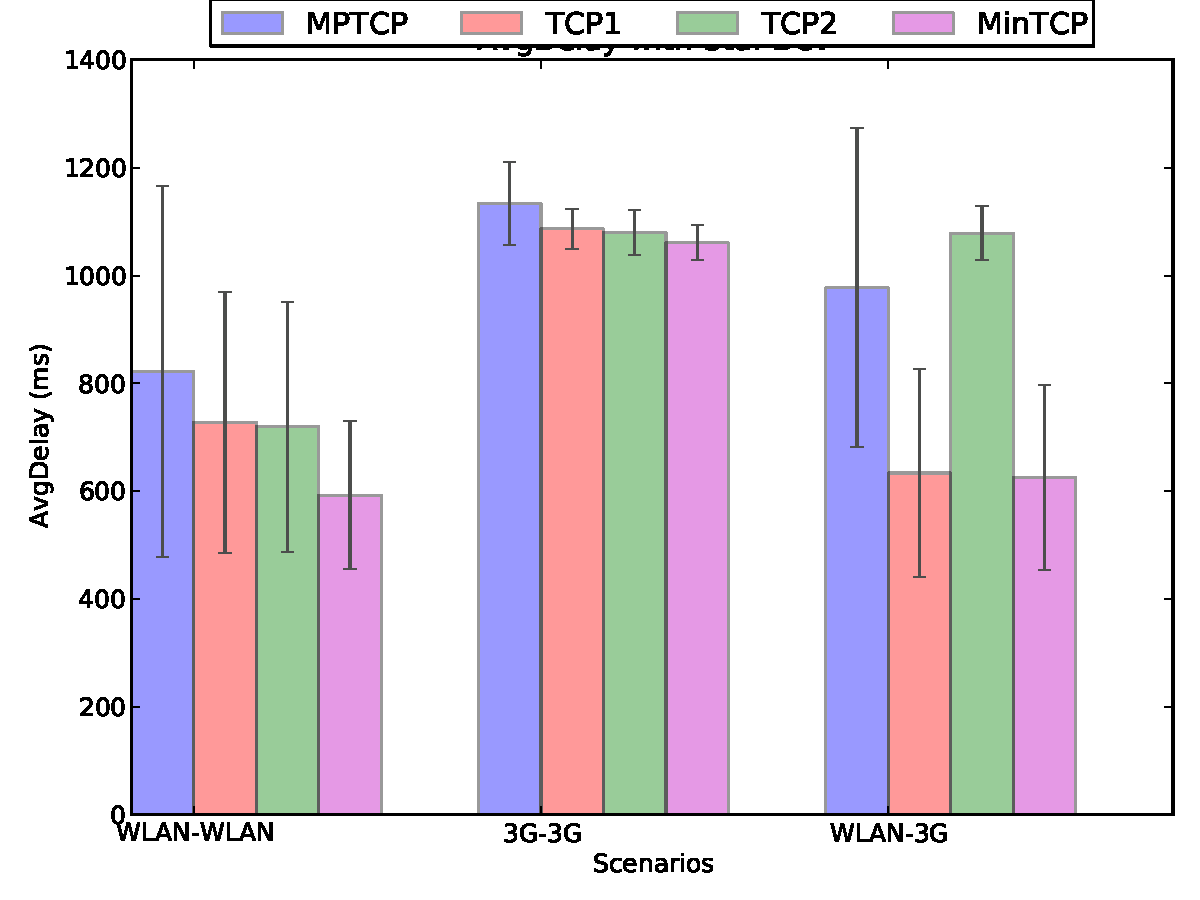
\includegraphics[width=.28\linewidth]{plots/Wikipedia_avgDelay_bar}
  } &
  \subfloat[Amazon download, $54$ objects, $1$Mb total size.\label{fig:web:amazon}]
  {
    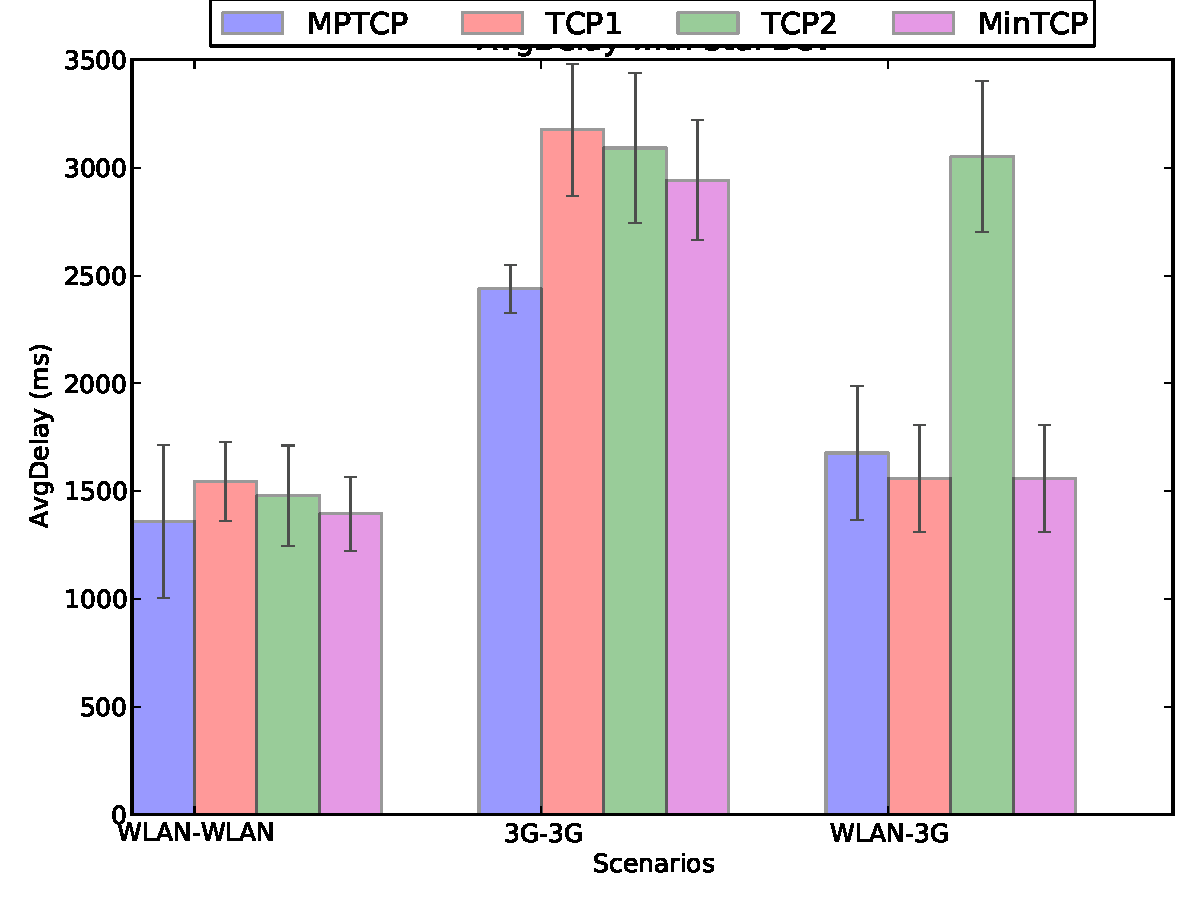
\includegraphics[width=.28\linewidth]{plots/Amazon_avgDelay_bar}
  } &
  \subfloat[Huffington Post download, $134$ objects, $3.9$Mb total size.\label{fig:web:huffpost}]
  {
    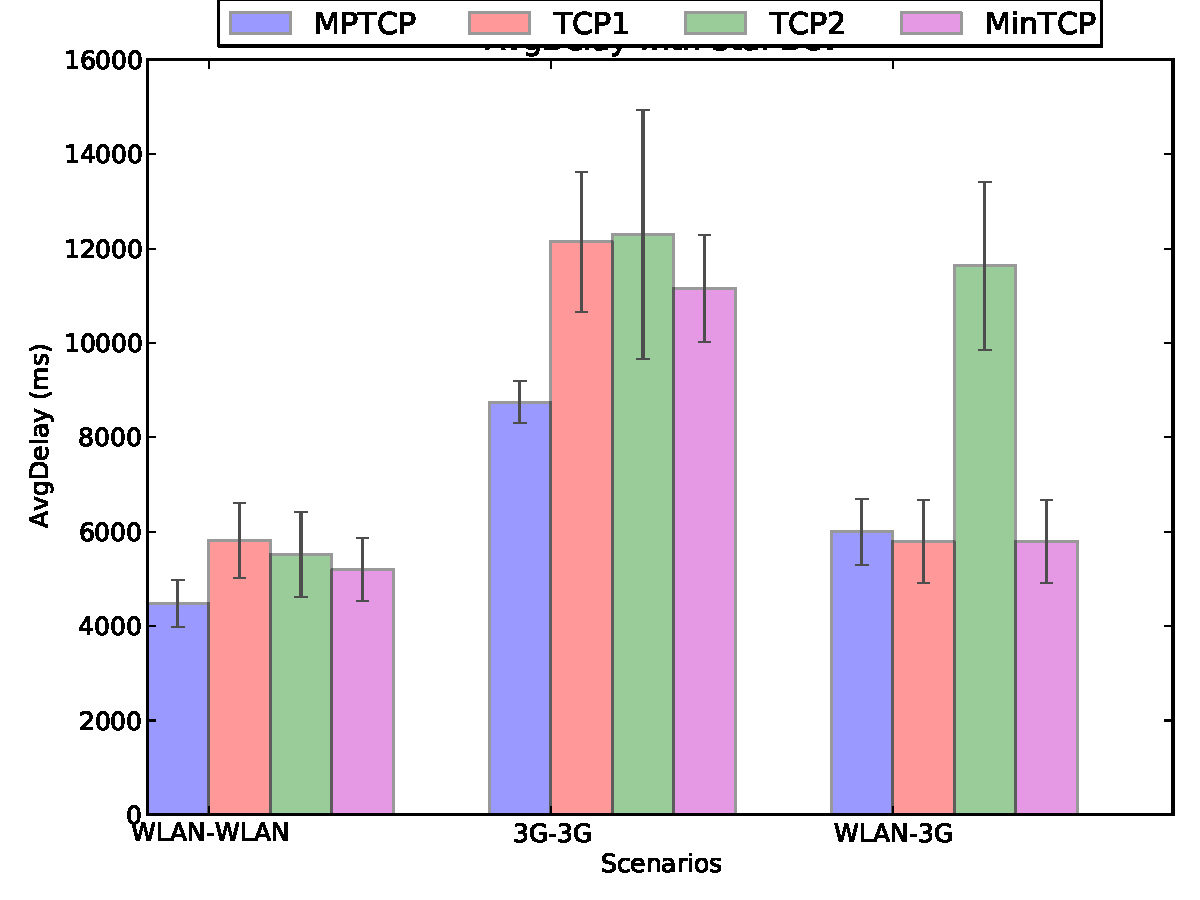
\includegraphics[width=.28\linewidth]{plots/Huffpost_avgDelay_bar}
  } 
%  \\
%  \subfloat[Wikipedia download, XYZ objects of average size XYZKB.\label{fig:web:wikipediawbg}]{
%	  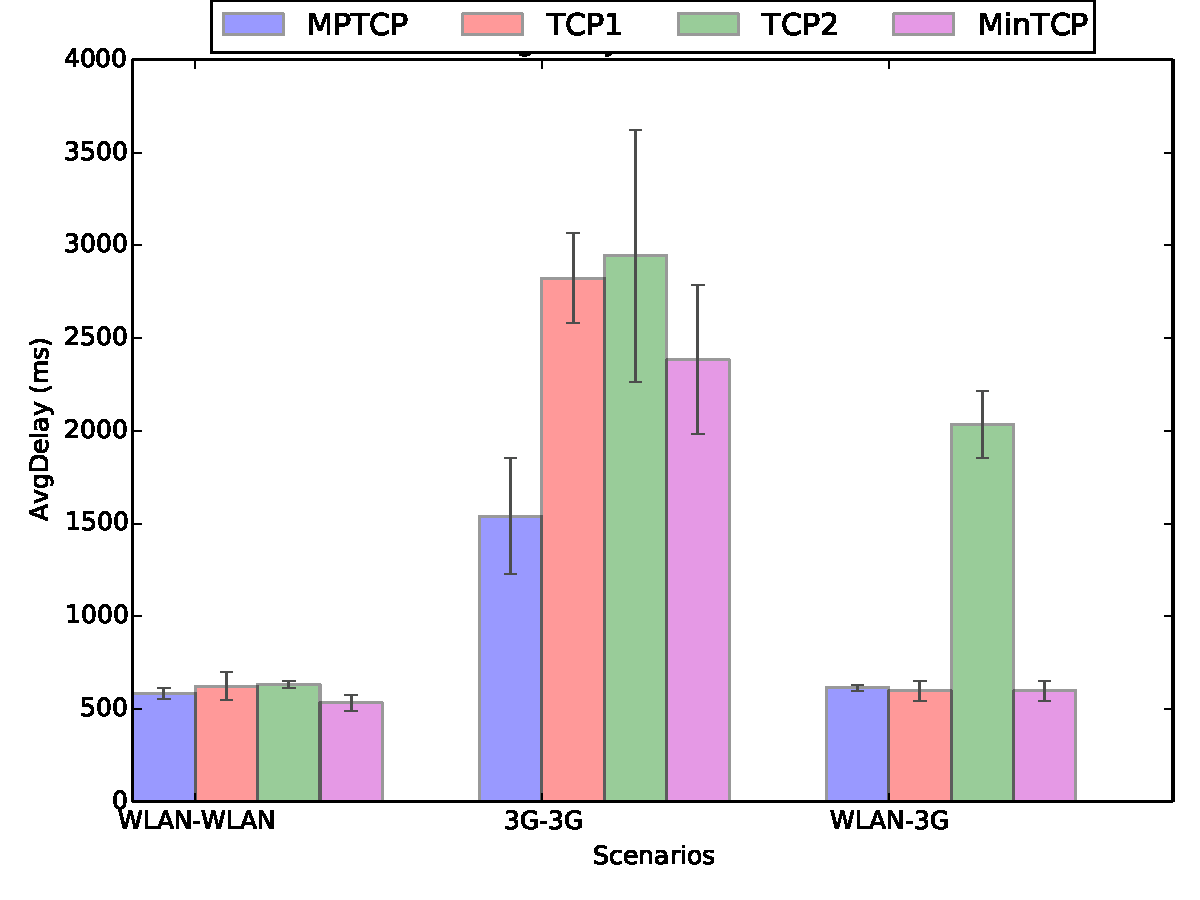
\includegraphics[width=.32\linewidth]{plots/wikipedia_avgDelayWBG}
%  } &
%  \subfloat[Amazon download, XYZ objects of average size XYZKB.\label{fig:web:amazonwbg}]
%  {
%    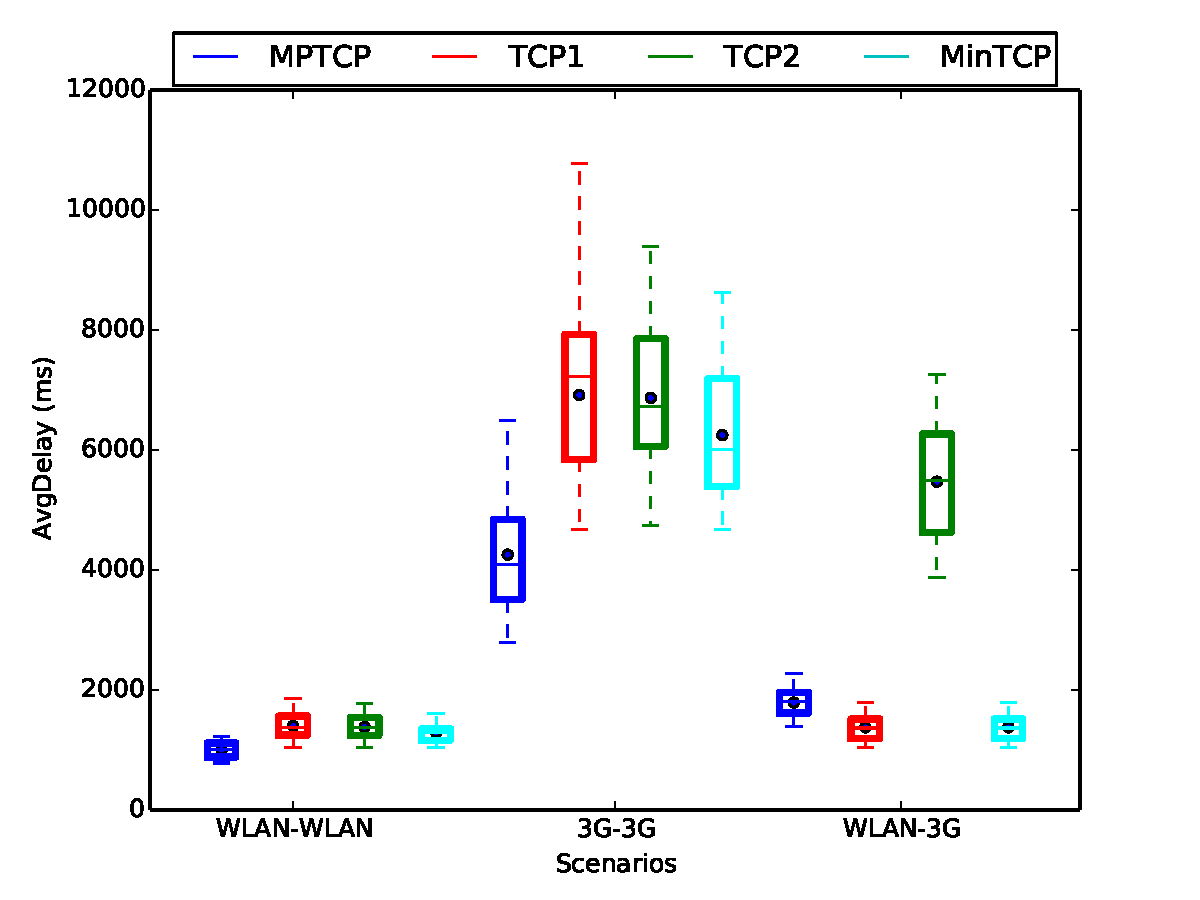
\includegraphics[width=.32\linewidth]{plots/Amazon_avgDelayWBG}
%  } &
%  \subfloat[Huffington Post download, XYZ objects of average size XYZKB.\label{fig:web:huffpostwbg}]
%  {
%    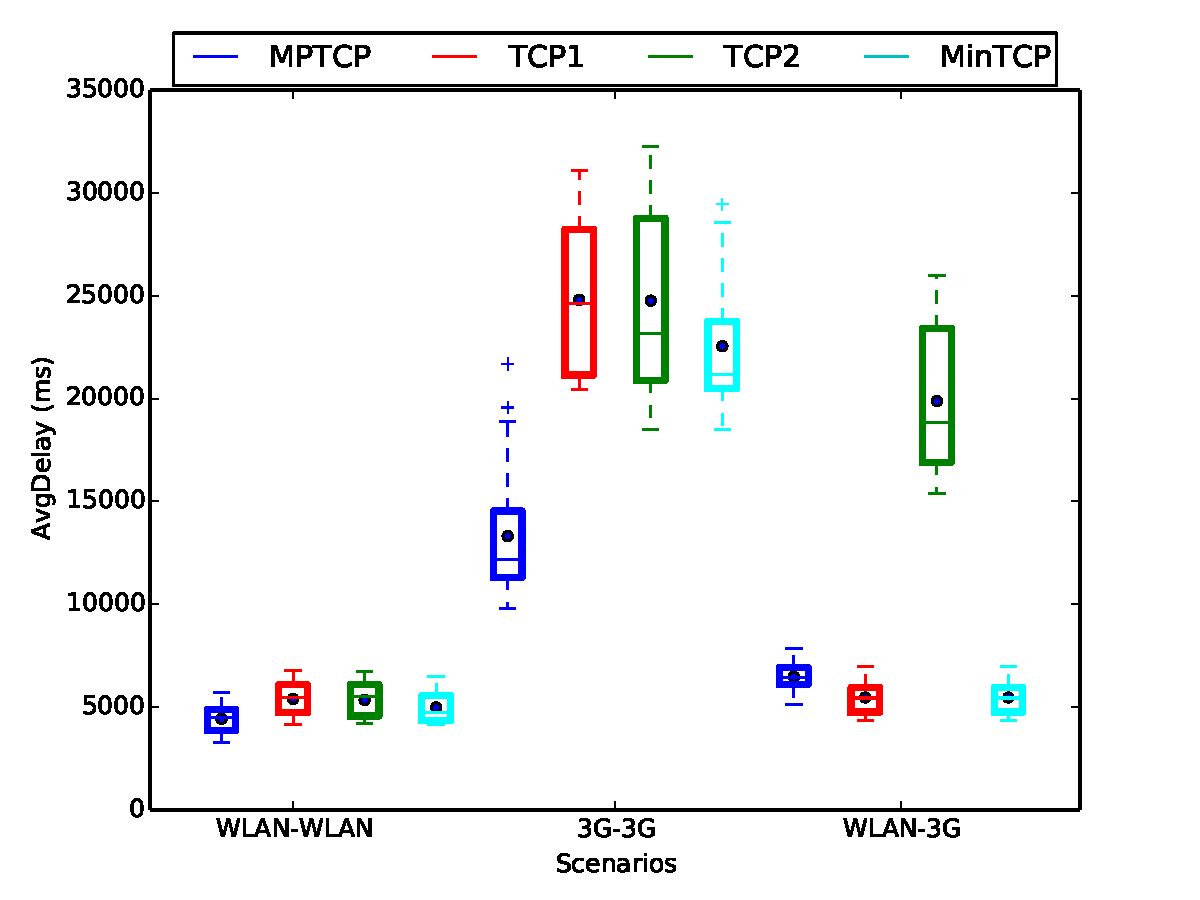
\includegraphics[width=.32\linewidth]{plots/huffpost_avgDelayWBG}
%  }
  \end{tabular}
  \caption{Average web transfer delay, with standard deviation.}
  \label{fig:web}
\end{figure*}


\begin{figure*}
  \centering
  \begin{tabular}{ccc}
  \subfloat[Wikipedia download, $15$ objects, $72$Kb total size.\label{fig:web:wikipedia-bg}]{
   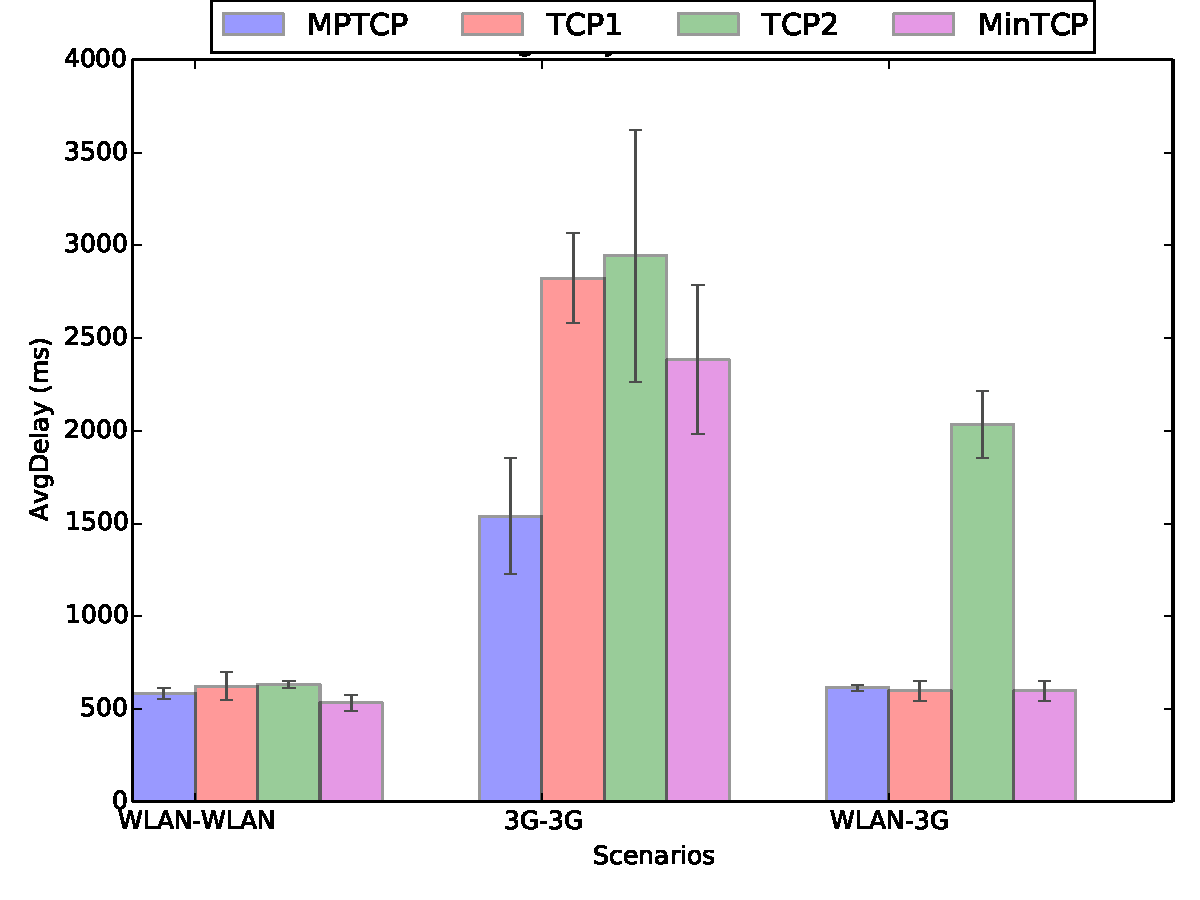
\includegraphics[width=.28\linewidth]{plots/wikipedia_avgDelayWBG}
  } &
  \subfloat[Amazon download, $54$ objects, $1$Mb total size.\label{fig:web:amazon-bg}]
  {
    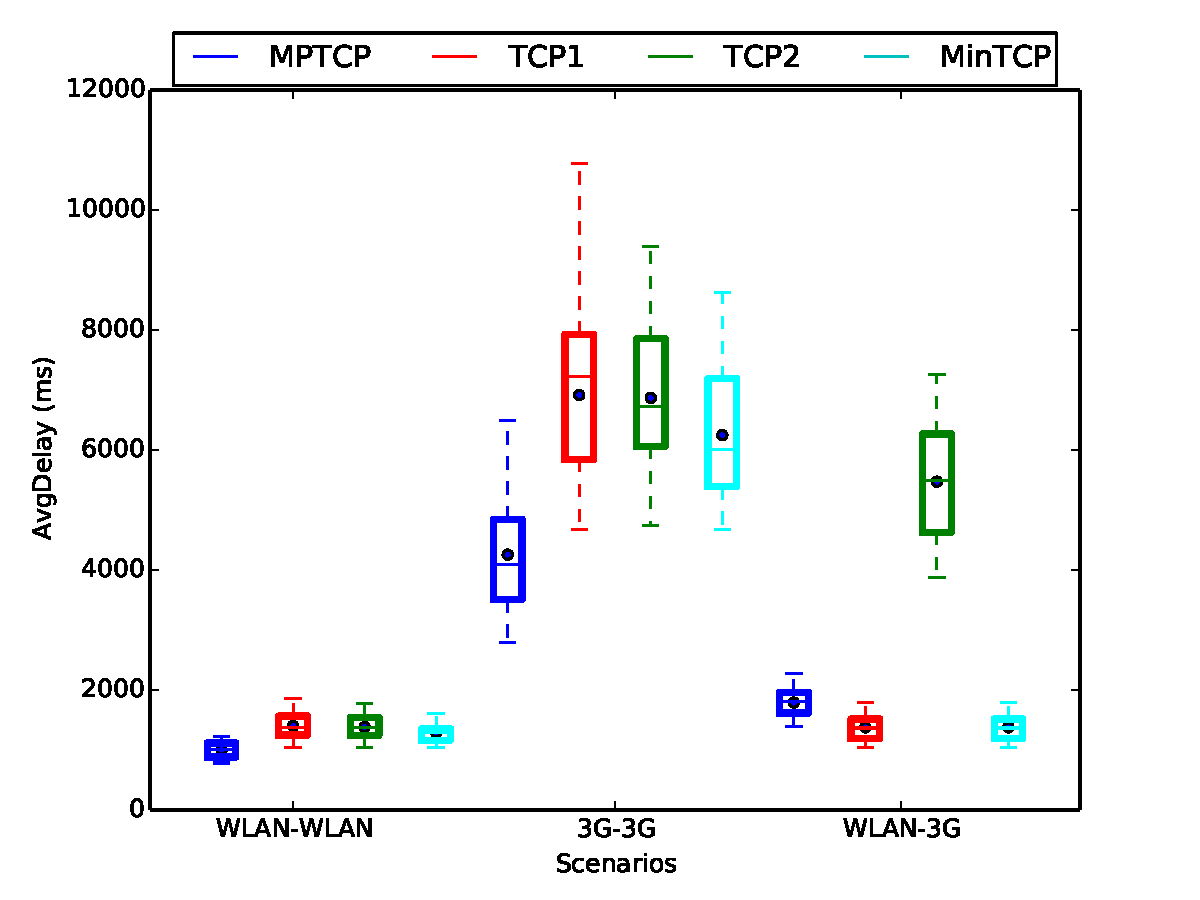
\includegraphics[width=.28\linewidth]{plots/Amazon_avgDelayWBG}
  } &
  \subfloat[Huffington Post download, $134$ objects, $3.9$Mb total size.\label{fig:web:huffpost-bg}]
  {
    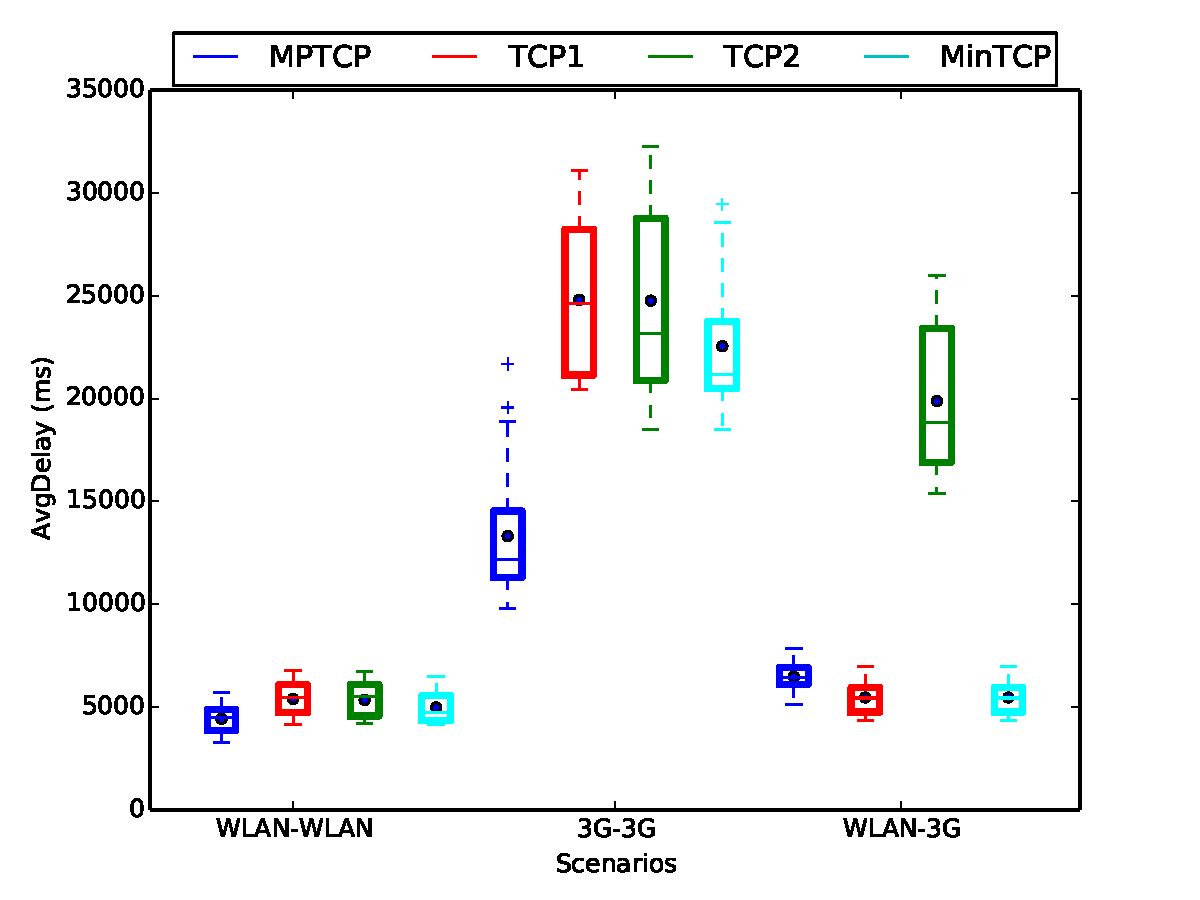
\includegraphics[width=.28\linewidth]{plots/huffpost_avgDelayWBG}
  }
 \end{tabular}
  \caption{With background flows: Average web transfer delay, with standard deviation.}
  \label{fig:web-bg}
\end{figure*}



Figure~\ref{fig:web} shows the average transfer times for web traffic, with standard variation over $30$ repetitions for 
each configuration without background traffic. Each figure depicts the average transfer time when using MPTCP, 
TCP on one of the interfaces (TCP1, TCP2), or TCP on the best available interface (MinTCP); the results are grouped according
to the emulated access networks used (WLAN-WLAN/3G-3G/WLAN-3G). We observe that MPTCP cannot reduce transfer times for the Wikipedia site, 
but is able to do so for both Amazon and Huffpost (especially in the 3G-3G scenarios). The reason for the poor performance of retrieving 
the Wikipedia site is simply that the amount of data is so small that it can be transmitted within TCP's initial window (given the six 
concurrent connections used). Employing more paths in such scenarios is not useful as long as the path itself can sustain the traffic load. 
However, for the other sites the amount of data is much larger and the transfer time can be reduced by MPTCP's implicit load-balancing over 
its available subflows; the positive effects of this load-balancing peek when the path characteristics of the subflows are homogeneous, as 
possible head-of-line blocking effects are less prevalent.


Figure \ref{fig:web-bg} illustrates the average transfer times for web traffic for emulations conducted with background traffic. 
For Wikipedia, with background traffic the results show similar behavior in WLAN-WLAN scenario as that of the no background case. 
There is substantial improvement in the download time in 3G-3G scenario. We observed losses in background flows in WLAN-WLAN and not in the 
3G-3G scenario. The WLAN access network settings further adds 1-2\% loss in the foreground traffic which could create head of line blocking. 
On the contrary 3G-3G scenario has no losses in the access network that improved downlowd times. In the asymmetric scenario (WLAN-3G) the performance 
of MPTCP is not significantly lower than that of the TCP as seen in no background case. We observed two different aspects that could be reason 
for this improvement. Primarily there were losses in the background flows that make the background TCP flow to back off at times. We also observed 
that data split between the two interfaces is not even, and more than 99\% of data transferred on the WLAN interface resulting in lower head of line blocking.

\begin{figure*}
  \centering
  \begin{tabular}{ccc}
  \subfloat[WLAN-WLAN Scenario packet path split.\label{fig:web:pshare-wlan-wlan}]{
   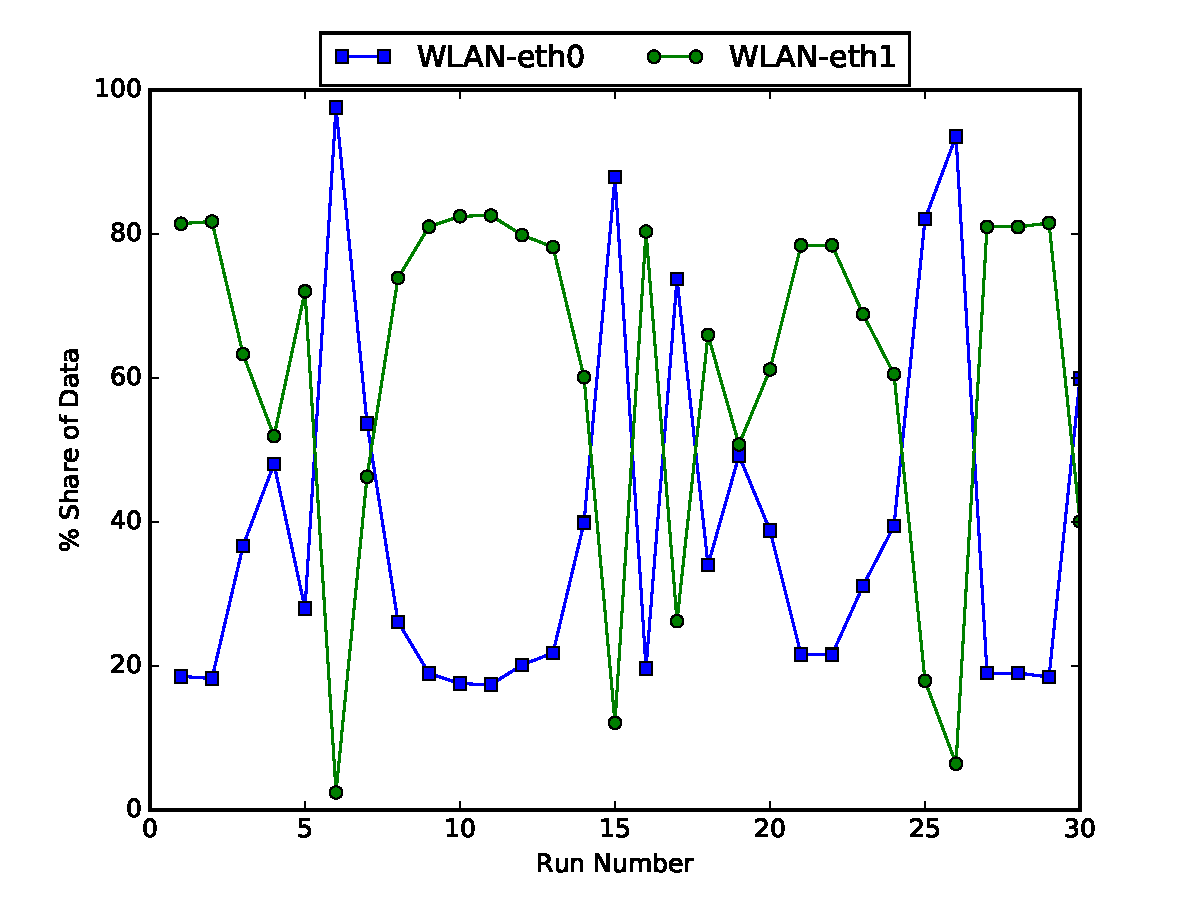
\includegraphics[width=.28\linewidth]{plots/pshare-WLAN-WLAN}
  } &
  \subfloat[3G-3G Scenario packet path split. \label{fig:web:pshare-3g-3g}]
  {
    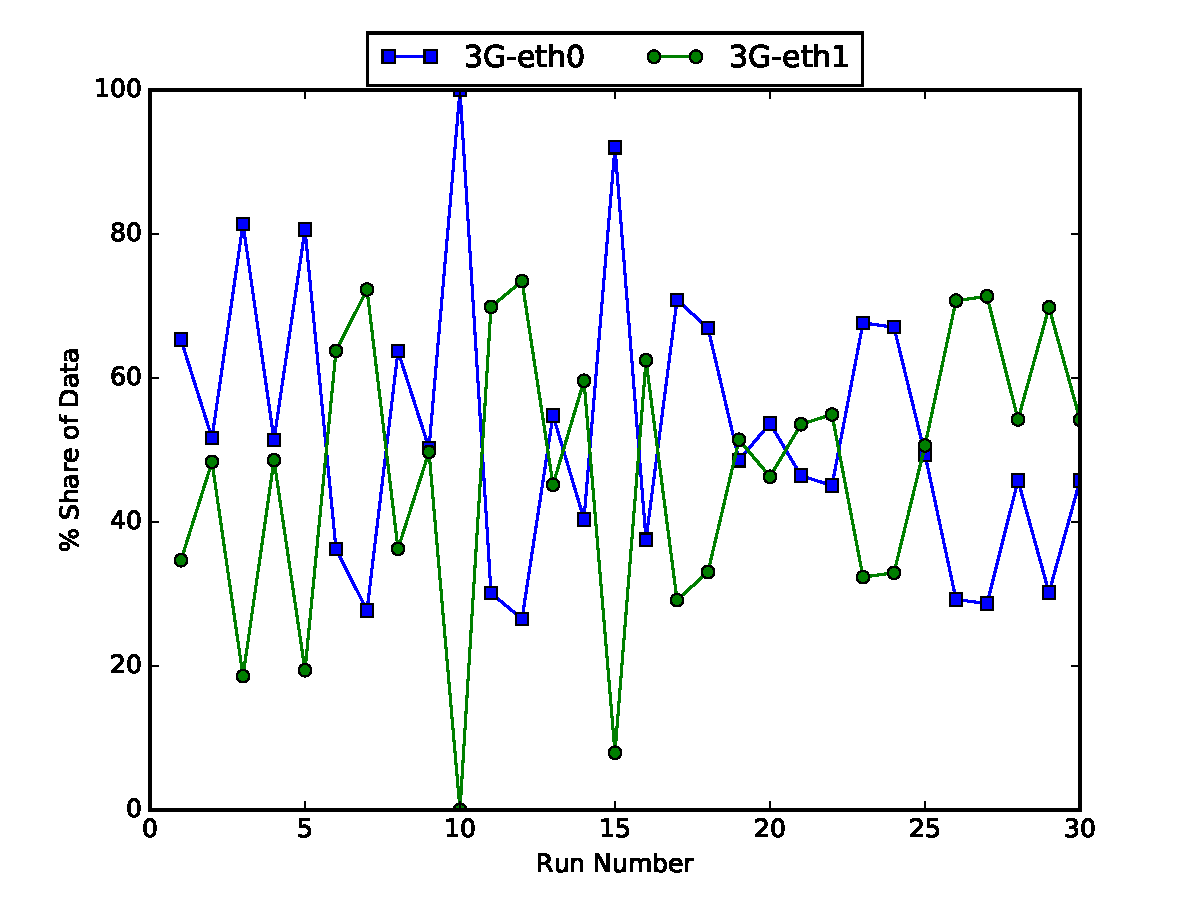
\includegraphics[width=.28\linewidth]{plots/pshare-3G-3G}
  } &
  \subfloat[WLAN-3G Scenario packet path split. \label{fig:web:pshare-wlan-3g}]
  {
    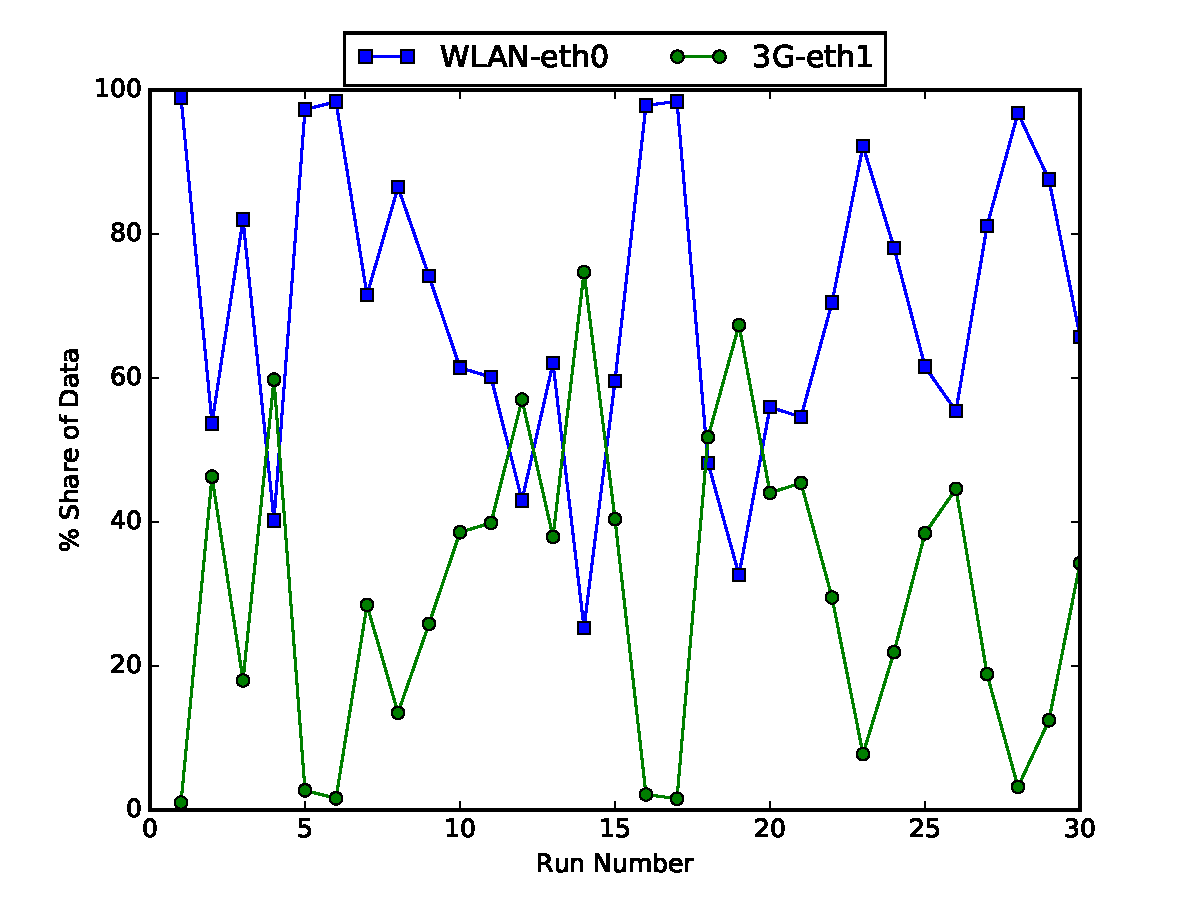
\includegraphics[width=.28\linewidth]{plots/pshare-WLAN-3G}
  }
 \end{tabular}
  \caption{MPTCP percent packets on each path without background traffic}
  \label{fig:web-pshare}
\end{figure*}

\begin{figure*}
  \centering
  \begin{tabular}{ccc}
  \subfloat[WLAN-WLAN Scenario packet path split.\label{fig:web:pshare-wlan-wlan-bg}]{
   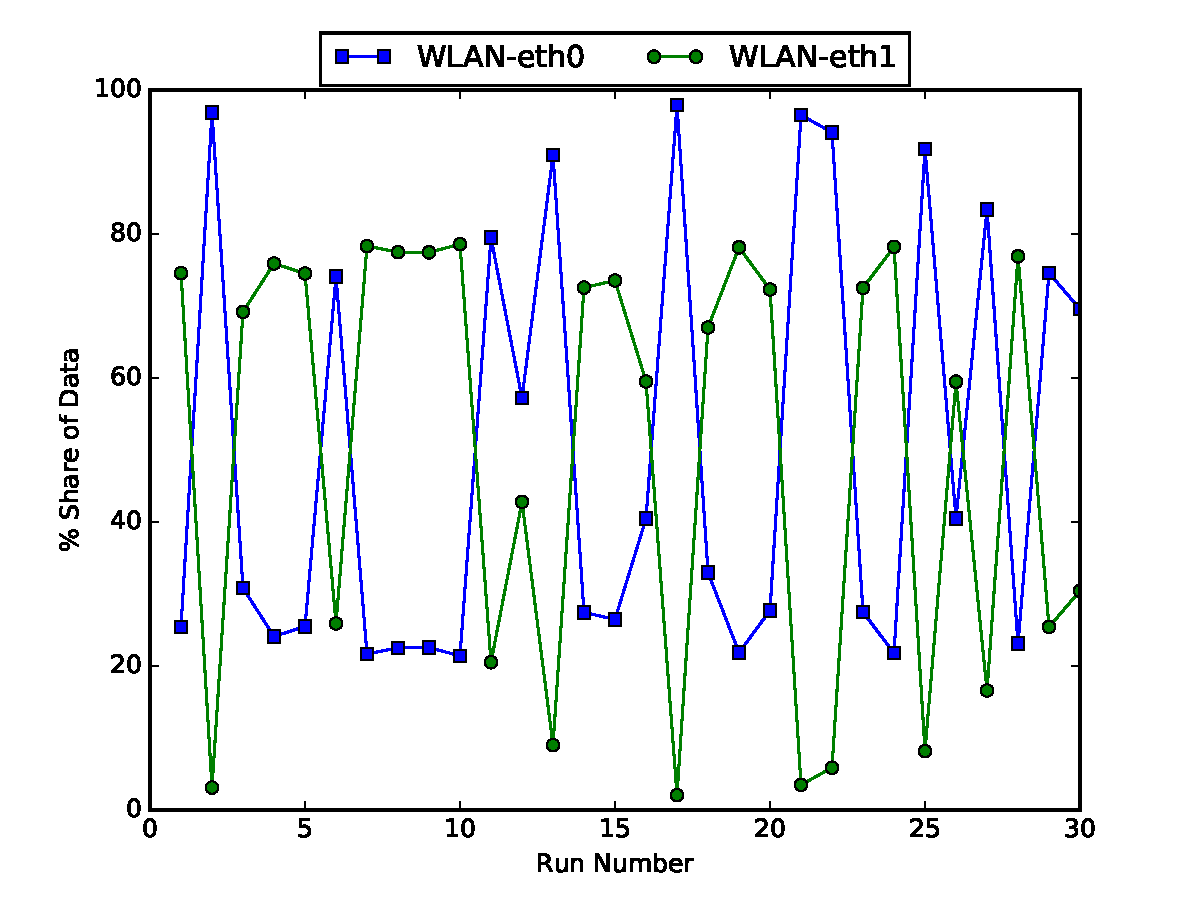
\includegraphics[width=.28\linewidth]{plots/pshare-WLAN-WLAN-BG}
  } &
  \subfloat[3G-3G Scenario packet path split. \label{fig:web:pshare-3g-3g-bg}]
  {
    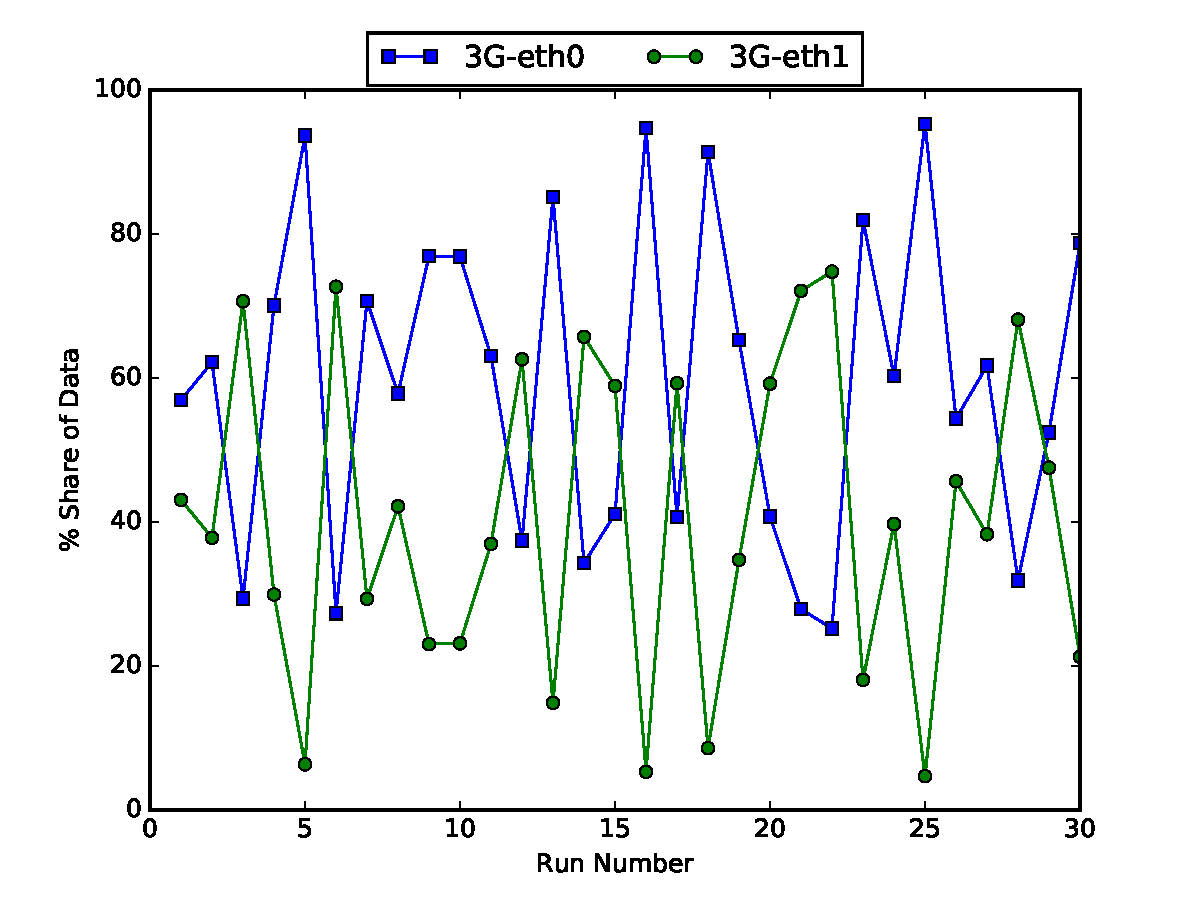
\includegraphics[width=.28\linewidth]{plots/pshare-3G-3G-BG}
  } &
  \subfloat[WLAN-3G Scenario packet path split. \label{fig:web:pshare-wlan-3g-bg}]
  {
    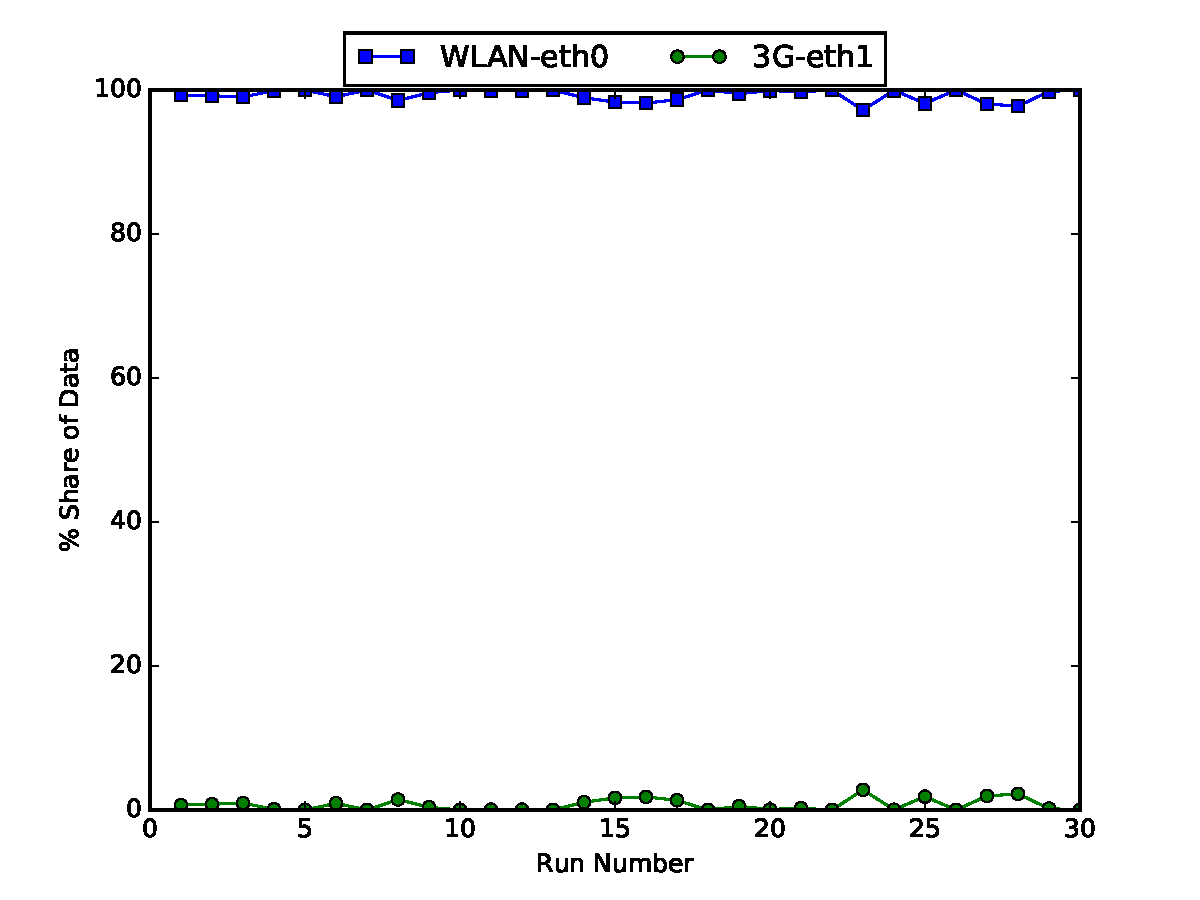
\includegraphics[width=.28\linewidth]{plots/pshare-WLAN-3G-BG}
  }
 \end{tabular}
  \caption{MPTCP percent packets on each path with background traffic}
  \label{fig:web-pshare-bg}
\end{figure*}

For Amazon and Huffpost, we observe similar behavior for no background and with background traffic cases in all the three scenairos. 
As expected, the download times are higher in the background case due to competing flows. 

\begin{figure}[!th]
\begin{minipage}[t]{0.48\textwidth}
\begin{center}
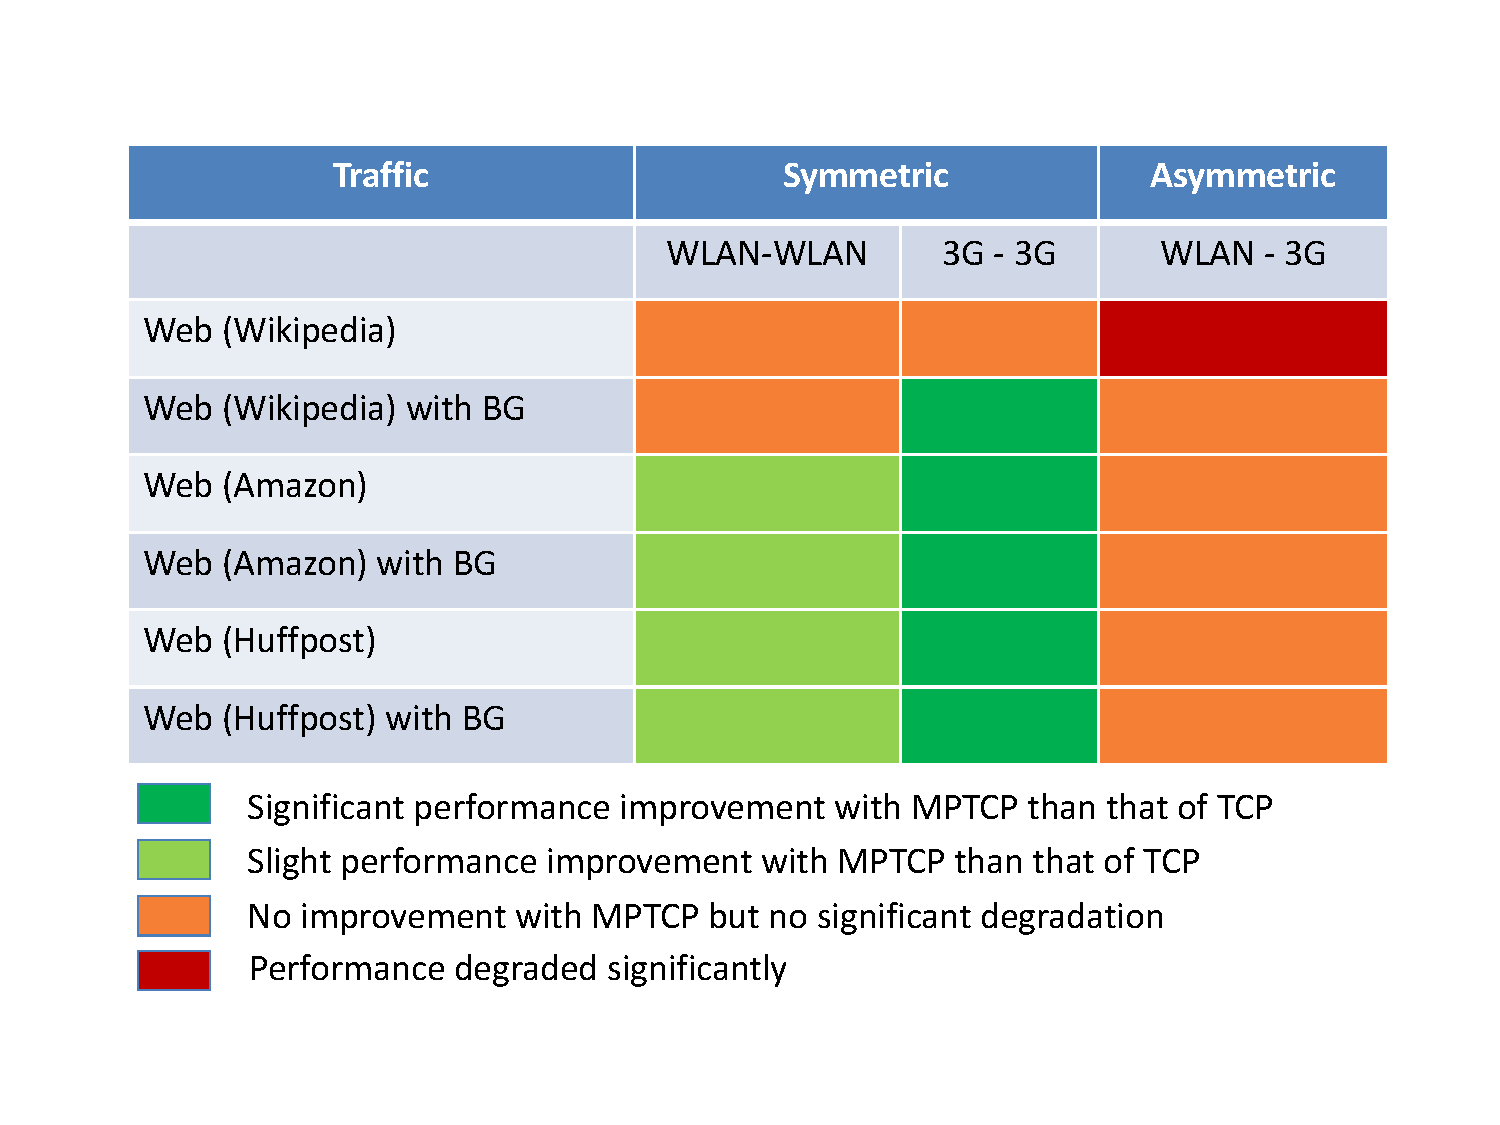
\includegraphics[width=.98\linewidth]{plots/MPTCP-Web}
\end{center}
\caption{Comparison of web traffic latency using MPTCP and TCP}
  \label{fig:web-summary}
\end{minipage}
\end{figure}

Further we analyze the percent share of traffic on each path for all scenarios. Figures~\ref{fig:web-pshare} and~\ref{fig:web-pshare-bg} reflects the 
share of data downloaded on each interface in no background traffic and with background traffic scenarios respectively. This analysis provides insight
in understanding the improvement or degradation of performance in the operational use of MPTCP in all scenarios. In the case of no background traffic,
the data is split between two paths for all scenarios. This is due to the fact that there is not enough data to transfer compared to the capacity of the
link. The packet scheduler of MPTCP uses the path with lowest RTT in its default setting. WLAN being signficantly faster than 3G, should transfer more share 
of data in asymmetric sceario. But the considerable split of data usage on 3G is due to the losses in WLAN and some of the flows being extremely
slow to wait for the WLAN RTT estimate recovery after loss.

With background traffic, the percent share of data is similar to that of the no background in symmetric scenarios with significant split between paths.
In asymmetric case, most of the data is transfered on WLAN and very little data is seen in 3G. This is due to multiple reasons including not enough data 
to transfer at WLAN rates making it impossible to switch to 3G, losses in the background flows, and no losses in the foreground flows.

In this paper, we considered different cases to observe the performance of MPTCP in terms of web traffic latency. We believe it is extremely important to
summarize our results in a form of systematic comparison to reduce presentation complexity. In Figure \ref{fig:web-summary} we provide a comparison 
chart of web traffic latency in using MPTCP and TCP across all scenarios. This chart covers all the cases emulated and the corresponding observations where $BG$ 
signifies with Background traffic. 


% ###########################################################################
\section{Conclusion}
\label{sec:conclusion}
% ###########################################################################

In this paper, we evaluate the latency performance of MPTCP in web traffic with that of TCP using emulations. We observed that MPTCP utilizes the 
available paths efficiently when there is enough data to send and performs better when there is path symmetry. No improvement with MPTCP was observed
when there is path asymmetry and it performs worse when there is not enough data to send. Moreover, our results indicate that MPTCP provides significant 
gains for websites with large object sizes both for homogeneous and heterogeneous paths. Further studies are planned to understand the congestion response 
of MPTCP in these traffic conditions. 




%The issues encountered by MPTCP are located at various level and local solutions
%may be provided to solve specific problems. In this paper, we list these
%problems to highlight that improving the performance of MPTCP is a complex task.
%We believe that the deployment of MPTCP must be considered in regards with the
%application profile and the very latest versions of single-path TCP.   



% ###########################################################################
%\section*{Acknowledgments}
% ###########################################################################

%The authors are funded by the European Community under its Seventh Framework
%Programme through the Reducing Internet Transport Latency~(RITE)
%project~(ICT-317700). The views expressed are solely those of the authors.

%\per{the references looks messy, might need a bit of a cleanup}

\bibliographystyle{IEEEtran}
\bibliography{references}

\end{document}
